\documentclass[11pt,a4paper]{report}

\PassOptionsToPackage{hypertexnames=false}{hyperref}
% shared/macros.tex
% Shared notation for all surface-partition math documents.
% Include with: \input{../shared/macros}

% -------------------------------------------------------------------------
% Packages (include here so each document only needs \input{../shared/macros})
% -------------------------------------------------------------------------
\usepackage{amsmath,amssymb,amsthm}
\usepackage{bm}           % \bm for bold math
\usepackage{mathtools}    % \coloneqq, dcases, etc.
\usepackage{booktabs}     % \toprule etc. in tables
\usepackage{hyperref}
\usepackage{geometry}
\usepackage{microtype}
\usepackage{parskip}
\usepackage{xcolor}
\usepackage{tcolorbox}
\usepackage{enumitem}
\usepackage{float}             % [H] float placement

\geometry{a4paper, margin=2.5cm}

% -------------------------------------------------------------------------
% Theorem-like environments
% -------------------------------------------------------------------------
\theoremstyle{definition}
\newtheorem{defn}{Definition}[section]
\newtheorem{remark}{Remark}[section]

\theoremstyle{plain}
\newtheorem{prop}{Proposition}[section]

% -------------------------------------------------------------------------
% Mesh and geometry
% -------------------------------------------------------------------------
\newcommand{\V}{\mathbf{V}}            % vertex array V[i] in R^dim
\newcommand{\F}{\mathbf{F}}            % face (triangle) array
\newcommand{\vone}[1]{v_{1,#1}}       % first vertex index of VP i
\newcommand{\vtwo}[1]{v_{2,#1}}       % second vertex index of VP i

% -------------------------------------------------------------------------
% Variable points
% -------------------------------------------------------------------------
\newcommand{\lam}{\lambda}             % scalar VP parameter
\newcommand{\Lam}{\boldsymbol{\lambda}}% full parameter vector
\newcommand{\vp}[1]{\mathbf{p}_{#1}}  % 3D position of VP i
\newcommand{\ed}[1]{\mathbf{d}_{#1}}  % edge direction d_i = V[v1_i] - V[v2_i]

% -------------------------------------------------------------------------
% Steiner / triple-point
% -------------------------------------------------------------------------
\newcommand{\Sv}{\mathbf{S}}           % Steiner (Fermat-Torricelli) point
\newcommand{\Ki}{K_{i}}               % projection matrix (I-n_i n_i^T)/r_i
\newcommand{\Mmat}{M}                 % sum of K_i matrices at a triple point

% -------------------------------------------------------------------------
% Normals and unit vectors
% -------------------------------------------------------------------------
\newcommand{\nhat}{\hat{\mathbf{n}}}  % unit normal to a triangle
\newcommand{\Dhat}{\hat{\boldsymbol{\Delta}}}  % unit segment direction

% -------------------------------------------------------------------------
% Operations
% -------------------------------------------------------------------------
\newcommand{\norm}[1]{\left\|#1\right\|}
\newcommand{\abs}[1]{\left|#1\right|}
\newcommand{\ip}[2]{\langle #1,\, #2 \rangle}

% Projection perpendicular to a unit vector \uhat
\newcommand{\Proj}[1]{\bigl(\mathbf{I} - #1 #1^\top\bigr)}

% argmax operator (winner-take-all assignment in Phase 1 documents)
\DeclareMathOperator*{\argmax}{arg\,max}
\DeclareMathOperator*{\argmin}{arg\,min}

% -------------------------------------------------------------------------
% Calculus shorthands
% -------------------------------------------------------------------------
\newcommand{\pd}[2]{\dfrac{\partial #1}{\partial #2}}
\newcommand{\pdd}[3]{\dfrac{\partial^2 #1}{\partial #2\,\partial #3}}
\newcommand{\grad}{\nabla}
\newcommand{\Hess}[1]{\nabla^2 #1}

% -------------------------------------------------------------------------
% Optimization problem objects
% -------------------------------------------------------------------------
\newcommand{\Preg}{P_{\mathrm{reg}}}  % regular perimeter
\newcommand{\Pst}{P_{\mathrm{st}}}   % Steiner perimeter
\newcommand{\Areg}{A^{\mathrm{reg}}} % regular cell area
\newcommand{\Ast}{A^{\mathrm{st}}}   % Steiner area contribution
\newcommand{\Atgt}{\bar{A}}           % target area per cell
\newcommand{\Lagr}{\mathcal{L}}       % Lagrangian
\newcommand{\objfac}{\sigma}          % IPOPT objective scaling factor

% -------------------------------------------------------------------------
% Code cross-references (for "In the code..." callouts)
% -------------------------------------------------------------------------
\newcommand{\code}[1]{\texttt{#1}}
\newcommand{\codefile}[1]{\texttt{\small #1}}

% -------------------------------------------------------------------------
% Threshold dynamics / approach B (10-mbo-auction-dynamics)
% -------------------------------------------------------------------------
\newcommand{\Dlump}{D}                 % lumped mass matrix diag(v)
\newcommand{\Atau}{A_\tau}             % discrete diffusion operator (M + tau K)^{-1} M
\newcommand{\Etau}{E_\tau}             % heat-content (threshold-dynamics) energy
\newcommand{\Rcell}{R_{\mathrm{cell}}} % radius of the equal-area disc sqrt(Abar/pi)
\newcommand{\hmean}{h_{\mathrm{mean}}} % mean edge length
\newcommand{\hmax}{h_{\mathrm{max}}}   % max edge length
\newcommand{\Gt}{G_t}                  % heat kernel at time t
\newcommand{\Ktau}{K^{\mathrm{res}}_\tau} % resolvent (backward-Euler) kernel

\usepackage{graphicx}

\hypersetup{
  colorlinks = true,
  linkcolor  = blue!60!black,
  citecolor  = green!50!black,
  urlcolor   = blue!60!black,
  pdftitle   = {A Study Companion to Threshold Dynamics},
  pdfauthor  = {surface-partition project}
}

% -------------------------------------------------------------------------
% Boxes used throughout. Each has one job, so a reader can skip by colour.
% -------------------------------------------------------------------------
\newtcolorbox{keyidea}[1][]{colback=yellow!6!white, colframe=orange!60!black,
  fontupper=\small, title={Key idea}, #1}
\newtcolorbox{physics}[1][]{colback=green!4!white, colframe=green!40!black,
  fontupper=\small, title={Physics corner}, #1}
\newtcolorbox{codebox}[1][]{colback=blue!4!white, colframe=blue!40!black,
  fontupper=\small, title={In our code}, #1}
\newtcolorbox{numbersbox}[1][]{colback=gray!6!white, colframe=gray!50!black,
  fontupper=\small, title={Where the numbers come from}, #1}

\newcommand{\R}{\mathbb{R}}

\title{\textbf{A Study Companion to Threshold Dynamics}\\[0.5em]
  \large From the heat equation to volume-constrained auction dynamics,\\
  and how each idea appears in \codefile{src/partition/mbo\_auction.py}}
\author{}
\date{Started October 2026}

\begin{document}
\sloppy
\maketitle

\begin{abstract}
A learning document, written while reading the papers behind approach~B
(\codefile{docs/explanations/reading\_path\_for\_a\_collaborator.md}). It is aimed
at a reader trained in physics and applied mathematics who wants the
\emph{intuition} behind each method well enough to read the implementation, not
the proofs. Each chapter builds one idea from what a physicist already knows,
works the key derivation by hand, checks it with a small numerical experiment,
and ends by mapping the idea onto our code. The rigorous account of the method
as implemented is \codefile{docs/math/10-mbo-auction-dynamics/}; this document is
the road to it.
\end{abstract}

\tableofcontents

\chapter*{How to use this document}
\addcontentsline{toc}{chapter}{How to use this document}

\textbf{Order.} The chapters follow the reading path: the unconstrained scheme
(threshold dynamics, Chapter~\ref{ch:mbo}), then the constraint that keeps cells
at equal area, then how the diffusion step is done on a triangulated surface,
then the assignment machinery. Each chapter says which pages of which paper it
prepares you for.

\begin{center}
\small
\begin{tabular}{@{}cp{0.47\linewidth}p{0.40\linewidth}@{}}
\toprule
Ch. & Topic & Papers it prepares \\
\midrule
1 & Diffusion-generated motion: the MBO scheme & MBO 1992, MBO 1994, Esedo\u{g}lu--Otto 2015 \S1--4 \\
2 & Constraints and prices: Lagrange multipliers, the shifted threshold & Ruuth--Wetton 2003 \\
3 & Auction dynamics: the equal-area step as an assignment problem & Jacobs--Merkurjev--Esedo\u{g}lu 2018, Bertsekas 1988 \\
4 & Diffusion on a triangulated surface, and other kernels & Dziuk--Elliott 2013, Garcia-Cardona et al.\ 2014, Esedo\u{g}lu--Jacobs 2017 \\
5 & The time step on a discrete domain & van Gennip et al.\ 2014 \\
\bottomrule
\end{tabular}
\end{center}
Only Chapter~1 is written; the rest is the plan, and will change as reading
suggests.

\textbf{Boxes.} \emph{Key idea} boxes state the one thing to remember.
\emph{Physics corner} boxes translate into language you already have; skip them
if the translation is obvious. \emph{In our code} boxes say where the idea lives
in the repository. \emph{Where the numbers come from} boxes give the script that
regenerates every computed number and figure in the chapter.

\textbf{Reproducibility.} The repository rule applies here too: any number
produced by running code comes from a committed script under
\codefile{docs/study/scripts/} and its committed output under
\codefile{docs/study/data/}. Rebuild everything with \code{make -C docs/study
figures} and then \code{make -C docs/study}.

\textbf{Conventions.} The heat equation is $\partial_t u = \Delta u$ (diffusion
constant $D = 1$; the papers sometimes keep $D$). Its kernel at time $t$ in
$\R^d$ is
\[
  G_t(x) = (4\pi t)^{-d/2} e^{-|x|^2/4t},
\]
the density of a normal distribution with variance $2t$ in each coordinate. A
set $\Sigma$ has indicator $\chi_\Sigma$ (1 inside, 0 outside). Curvature
$\kappa$ is positive where a set is convex.

% Chapter 1 — the MBO primer.
% Numbers: docs/study/data/ch01.yaml, written by docs/study/scripts/ch01_mbo.py.

\chapter{Diffusion-generated motion: the MBO scheme}
\label{ch:mbo}

\begin{keyidea}
Blur a set with the heat equation for a short time $\tau$, then keep the points
where the blurred value is at least $\tfrac12$. Repeat. The boundary of the set
moves inward at a speed equal to its curvature, and curvature flow is the
fastest way to shorten a boundary. With $N$ sets, blur each one and give every
point to the set whose blurred value is largest. Every step lowers an energy
that approximates the total boundary length, so this simple loop is a
perimeter minimiser. Approach~B is this loop, with one extra rule that keeps
the cell areas equal.
\end{keyidea}

\paragraph{What this chapter prepares you for.}
Merriman, Bence \& Osher 1992 \cite{merriman1992diffusion}, \S2--4 (pages 3--5
of the report): the scheme and the authors' own argument for why it works.
Merriman, Bence \& Osher 1994 \cite{merriman1994motion}: the multiphase version
(skim, mainly the figures). Esedo\u{g}lu \& Otto 2015 \cite{esedoglu2015threshold},
\S1--4: the energy view of \S\ref{sec:ch1-energy}--\ref{sec:ch1-descent}.
Afterwards, \codefile{docs/math/10-mbo-auction-dynamics/} \S4 should read as a
summary of things you already know.

\begin{numbersbox}
Every number and figure in this chapter is produced by
\codefile{docs/study/scripts/ch01\_mbo.py} and recorded in
\codefile{docs/study/data/ch01.yaml} (python 3.12.13, numpy 2.4.4, scipy 1.17.1,
matplotlib 3.10.8; the one random draw uses seed 20261002; about 20\,s to run).
There are two kinds of experiment. \emph{Gridless} ones (experiments A and D)
use the exact formula for a blurred disc, so they test the continuum analysis
with no discretisation error. \emph{Grid} ones (B, C and E) run the algorithm on
a periodic unit square, a flat torus, with the heat step done exactly by FFT.
\end{numbersbox}

% =========================================================================
\section{The problem the scheme solves}
\label{sec:ch1-problem}

Our goal is to cut a surface into $N$ cells of equal area so that the total
length of the cell boundaries is as small as possible. Leave the area
constraint aside for this chapter and ask the simpler question:
\emph{given a set, how do you change it so that its boundary gets shorter as
fast as possible?} The answer is a classical geometric flow, which
\S\ref{sec:ch1-curvature} derives. MBO is a surprisingly simple way to compute
it.

Two properties make the scheme attractive for our problem, and they are the
reason it replaced PGD:
\begin{enumerate}[nosep]
  \item The state is always a \emph{hard} partition: every point belongs to
        exactly one cell, at every step. There is no fuzzy density to be
        ``read out'' at the end, so the gap between the relaxed solution and
        the partition you finally extract, which broke PGD at high $N$, cannot
        appear (\codefile{docs/reference/winner\_take\_all\_partition\_gap.md}).
  \item One step costs one linear solve per cell, and no small parameter
        $\varepsilon$ has to resolve an interface on the mesh.
\end{enumerate}

% =========================================================================
\section{Ingredient 1: the heat equation as a blur}
\label{sec:ch1-heat}

Solve $\partial_t u = \Delta u$ in $\R^d$ starting from $u(\cdot, 0) = f$. The
solution at time $\tau$ is a convolution:
\begin{equation}
  u(x, \tau) = (G_\tau * f)(x) = \int_{\R^d} G_\tau(x - y)\, f(y)\, dy,
  \qquad
  G_\tau(x) = (4\pi\tau)^{-d/2} e^{-|x|^2/4\tau}.
  \label{eq:ch1-heat}
\end{equation}
In words, the new value at $x$ is a Gaussian-weighted average of the old values
within distance about $\sqrt\tau$ of $x$. These are the facts about $G_\tau$
used in this chapter and the next ones:

\begin{enumerate}[nosep]
  \item \textbf{It is a probability density}: $G_\tau \ge 0$ and $\int G_\tau = 1$.
        So if $0 \le f \le 1$ then $0 \le G_\tau * f \le 1$, and
        $G_\tau * 1 = 1$. Blurring an indicator gives a number between 0 and 1,
        which you can read as ``how much of the neighbourhood of $x$ is
        inside the set''.
  \item \textbf{Variance $2\tau$ per coordinate.} If $X \sim G_\tau$, then
        $\mathbb E[X_i^2] = 2\tau$. The blur radius is $\sqrt{2\tau}$ in each
        direction. This factor of 2 is where the 2 in $R^2 = R_0^2 - 2t$
        (\S\ref{sec:ch1-curvature}) comes from.
  \item \textbf{It is symmetric}: $G_\tau(x) = G_\tau(-x)$, so
        $\int f\, (G_\tau * g) = \int (G_\tau * f)\, g$.
  \item \textbf{Its Fourier transform is positive}:
        $\widehat{G_\tau}(\xi) = e^{-\tau|\xi|^2} > 0$. Blurring damps every
        wavelength and never reverses one. This is the property that makes
        the energy of \S\ref{sec:ch1-energy} concave.
  \item \textbf{Semigroup}: $G_s * G_t = G_{s+t}$. Blurring for $s$ and then
        for $t$ is the same as blurring for $s + t$.
\end{enumerate}

\begin{physics}
$u$ is a temperature, $f$ the initial temperature and $\tau$ the elapsed time
(with $D = 1$). Equivalently, $G_\tau * f$ is the expected value of $f$ seen by a
random walker started at $x$ after time $\tau$. When $f = \chi_\Sigma$, the
blurred value $(G_\tau * \chi_\Sigma)(x)$ is \emph{the probability that a
Brownian particle started at $x$ is inside $\Sigma$ at time $\tau$}. Both the
curvature result and the energy below are easiest to see in this picture.
\end{physics}

% =========================================================================
\section{Ingredient 2: curvature, and the flow that shortens curves}
\label{sec:ch1-curvature}

Take a closed curve in the plane, the boundary of a set $\Sigma$, with arc
length $s$. Its curvature $\kappa(s)$ is the rate at which the tangent direction
turns per unit length. A circle of radius $R$ has $\kappa = 1/R$, and a straight
line has $\kappa = 0$. We take $\kappa > 0$ where $\Sigma$ is locally convex.

\paragraph{How length changes when the curve moves.}
Push every point of the curve outward along the normal by a small distance
$\phi(s)$. To first order, the length changes by
\begin{equation}
  \delta L = \int \kappa\, \phi \, ds.
  \label{eq:ch1-first-variation}
\end{equation}
Check this on a circle: pushing it out uniformly by $\phi$ turns length $2\pi R$
into $2\pi(R + \phi)$, so $\delta L = 2\pi\phi = \int (1/R)\,\phi\, ds$. In
general, a curved piece of boundary is like a piece of a circle of radius
$1/\kappa$; pushing it outward lengthens it in proportion to $\kappa$, while
moving a straight piece changes nothing.

\paragraph{Steepest descent.}
Now let the curve move with outward normal velocity $V(s)$. Then
$dL/dt = \int \kappa V\, ds$. Among all velocity fields of a given size
$\int V^2 ds$, this rate is most negative for $V = -\kappa$: \emph{move every
point inward at a speed equal to its curvature}. That is \textbf{motion by
curvature} (curve-shortening flow), and along it
\begin{equation}
  \frac{dL}{dt} = -\int \kappa^2\, ds \;\le\; 0 .
  \label{eq:ch1-dLdt}
\end{equation}
Curvature flow is the gradient flow of length.

\paragraph{Two exact consequences, which the experiments will check.}
\begin{itemize}[nosep]
  \item \emph{Area falls at a constant rate.} $dA/dt = \int V\, ds =
        -\int \kappa\, ds = -2\pi$ for every simple closed curve, because the
        tangent turns through exactly $2\pi$ going once around. The rate does
        not depend on the shape.
  \item \emph{A disc stays a disc.} With $dR/dt = -1/R$,
        \begin{equation}
          R(t)^2 = R_0^2 - 2t, \qquad \text{extinct at } t^\ast = R_0^2/2 .
          \label{eq:ch1-disc}
        \end{equation}
\end{itemize}
In the plane, curve-shortening flow never pinches an embedded curve into two
pieces. Every such curve becomes convex and then shrinks to a round point
(Grayson's theorem \cite{grayson1987heat}). Experiment~C shows this. On a
surface the same flow is \emph{geodesic} curvature flow, and the formulas
change only through the surface's own curvature.

\begin{physics}
This is the law of motion of a grain boundary or a soap film, $v = \mu\sigma\kappa$
(mobility times surface tension times curvature), which Mullins wrote down for
idealised grain growth \cite{mullins1956two}. In a 2-D cellular network with
$120^\circ$ junctions it gives the von~Neumann--Mullins law: a cell with $n$
sides changes area at a rate proportional to $n - 6$. Cells with fewer than six
sides shrink, cells with more grow, and hexagons are neutral. Keep this in mind
for Chapter~3, where auction dynamics tiles a flat torus with hexagons.
\end{physics}

% =========================================================================
\section{The MBO algorithm}
\label{sec:ch1-algorithm}

\begin{tcolorbox}[colback=white, colframe=black!60, title={Two-phase MBO
  \cite{merriman1992diffusion}}, fontupper=\small]
Given a set $\Sigma^0$ and a time step $\tau$, repeat for $n = 0, 1, 2, \dots$:
\begin{enumerate}[nosep]
  \item \textbf{Diffuse:} $u = G_\tau * \chi_{\Sigma^n}$.
  \item \textbf{Threshold:} $\Sigma^{n+1} = \{x : u(x) \ge \tfrac12\}$.
\end{enumerate}
After $n$ steps the boundary approximates the curvature flow at time $t = n\tau$.
\end{tcolorbox}

The diffuse step is linear and cheap (an FFT on a grid, one sparse solve on our
mesh). The threshold step is pointwise. Nothing tracks the curve, so corners,
merging and topology changes need no special handling.

\begin{physics}
Think of it as a repeated quench: let heat spread for a short time, then quench
to zero temperature, so every point snaps to whichever phase is locally in the
majority. The physics of the interface (its motion by curvature) emerges from
the competition between the two operations. The interface itself is never
represented.
\end{physics}

% =========================================================================
\section{Why the boundary moves by curvature}
\label{sec:ch1-why}

\subsection{The argument in the 1992 paper}

MBO's own argument \cite[\S3]{merriman1992diffusion} is the one to read first.
At a boundary point $P$, use polar coordinates $(r, \theta)$ centred at the
centre of curvature of $P$, so $P$ is at $r = \rho = 1/\kappa$. The heat equation
reads
\[
  \partial_t \chi = \partial_{rr}\chi + \frac1r\,\partial_r\chi
                   + \frac{1}{r^2}\,\partial_{\theta\theta}\chi .
\]
Near $P$ the set is locally a disc around that centre, so $\theta$-derivatives
vanish and
\begin{equation}
  \partial_t \chi \;-\; \frac1r\,\partial_r \chi \;=\; \partial_{rr}\chi .
  \label{eq:ch1-advdiff}
\end{equation}
This is a one-dimensional \emph{advection--diffusion} equation. The left side
is transport toward the centre of curvature at speed $1/r = \kappa$. The right
side is plain 1-D diffusion, which smears the step symmetrically about its
midpoint and therefore does not move the level $\chi = \tfrac12$. So in a short
time $\tau$ the $\tfrac12$ level is carried a distance $\kappa\tau$ toward the
centre of curvature, and thresholding at $\tfrac12$ reads off exactly that
level. Figure~3 of the paper shows this picture: a step that advects and spreads.

\subsection{The same result from the Gaussian directly}

The polar argument is heuristic: the step is not smooth, and ``locally a disc''
needs care. A short computation makes it concrete, and it is the kind of
estimate the later papers use. Put $P$ at the origin with the set below a
parabola, $\Sigma = \{(x, y) : y < -\tfrac{\kappa}{2}x^2\}$ (convex for
$\kappa > 0$). Evaluate the blurred indicator at the point $(0, y_0)$. A 2-D
Gaussian is a product of two 1-D Gaussians $g_\tau$, each with variance $2\tau$,
so with $\Phi_\tau(z) = \int_{-\infty}^z g_\tau$,
\[
  u(0, y_0) = \Pr\bigl[\,y_0 + Y < -\tfrac{\kappa}{2} X^2\,\bigr]
            = \int g_\tau(x)\, \Phi_\tau\!\bigl(-\tfrac{\kappa}{2}x^2 - y_0\bigr)\, dx .
\]
The typical $x$ is of size $\sqrt\tau$, so the argument of $\Phi_\tau$ is of
size $\kappa\tau + |y_0|$. That is much smaller than the blur width $\sqrt\tau$
when $\kappa\sqrt\tau \ll 1$. So we may linearise,
$\Phi_\tau(z) \approx \tfrac12 + g_\tau(0)\, z$:
\[
  u(0, y_0) \approx \tfrac12 - g_\tau(0)\Bigl(\tfrac{\kappa}{2}\,\mathbb E[X^2] + y_0\Bigr)
            = \tfrac12 - g_\tau(0)\,\bigl(\kappa\tau + y_0\bigr).
\]
The new boundary, where $u = \tfrac12$, is at $y_0 = -\kappa\tau$. In one step the
boundary moves into the set by
\begin{equation}
  \boxed{\;\text{displacement} = \kappa\,\tau\,\bigl(1 + O(\kappa^2 \tau)\bigr)\;}
  \qquad\Longrightarrow\qquad V = \kappa .
  \label{eq:ch1-displacement}
\end{equation}
A flat interface ($\kappa = 0$) does not move at all: by symmetry its blurred
profile crosses $\tfrac12$ exactly at the old boundary.

\paragraph{Experiment A (gridless): the one-step displacement.}
For a disc of radius $R$, the blurred indicator at distance $r$ from the centre is
the probability that a normal vector with variance $2\tau$, started at distance
$r$, lands in the disc. This is a noncentral $\chi^2$ distribution function,
exact and with no grid. Figure~\ref{fig:ch1-displacement} (left) compares the
profile with that of a flat interface; the disc's profile crosses $\tfrac12$
inside the old boundary. Figure~\ref{fig:ch1-displacement} (right) plots the
exact displacement divided by $\kappa\tau$. The three radii fall on one curve
because, by dimensional analysis, the ratio can depend only on
$\sqrt\tau/R$. For $R = 0.2$ the ratio is $1.002$, $1.008$, $1.036$ and $1.209$ at
$\sqrt\tau/R = 0.05$, $0.1$, $0.2$ and $0.4$: equation
\eqref{eq:ch1-displacement} is exact in the limit, and the relative correction grows like
$(\sqrt\tau/R)^2 = \kappa^2\tau$ (it quadruples each time $\sqrt\tau/R$ doubles), as the
$O(\kappa^2\tau)$ in \eqref{eq:ch1-displacement} says. It has no term linear in
$\sqrt\tau/R$ because $\Phi_\tau$ has no quadratic term at its midpoint.

\begin{figure}[H]
  \centering
  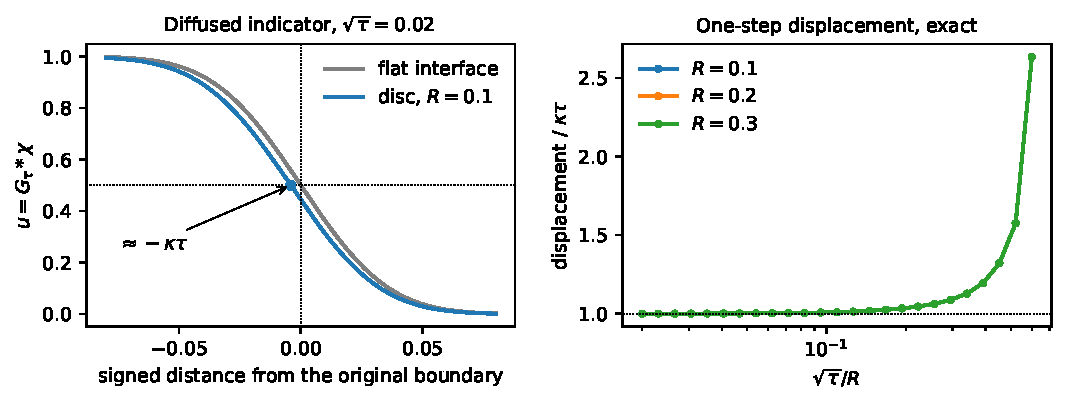
\includegraphics[width=\linewidth]{figures/ch01_displacement.pdf}
  \caption{Left: blurred indicator across a flat interface and across the
  boundary of a disc of radius 0.1, at $\sqrt\tau = 0.02$. The $\tfrac12$ crossing
  of the disc (dot) sits about $\kappa\tau$ inside the original boundary. Right:
  exact one-step displacement over $\kappa\tau$; the ratio tends to 1 as
  $\sqrt\tau/R \to 0$.}
  \label{fig:ch1-displacement}
\end{figure}

\paragraph{Experiment B (grid): a disc shrinking over many steps.}
On a $512 \times 512$ periodic grid ($h = 1/512 \approx 0.00195$), start from a
pixelated disc with $R_0 = 0.25$ and run MBO. Equation~\eqref{eq:ch1-disc}
predicts $R^2$ falling linearly to zero at $t^\ast = 0.03125$. With
$\tau = 10^{-3}$, Figure~\ref{fig:ch1-disc} shows the measured $R^2 = $ area$/\pi$
on that line: the disc vanishes at $t = 0.031$, and halfway through,
$R^2 = 0.0303$ against $0.0305$ predicted.

\paragraph{Experiment C (grid): a non-convex set.}
Figure~\ref{fig:ch1-dumbbell} runs MBO ($\tau = 5\times 10^{-4}$) on a disc and a
square joined by a bar. Corners round off immediately, concave corners fill in,
the shape becomes convex as Grayson's theorem predicts, and the area falls at
the shape-independent rate $2\pi \approx 6.28$. The measured mean rate is $6.47$ up
to $t = 0.008$ and $6.49$ up to $t = 0.016$, within 3\%.

\begin{figure}[H]
  \centering
  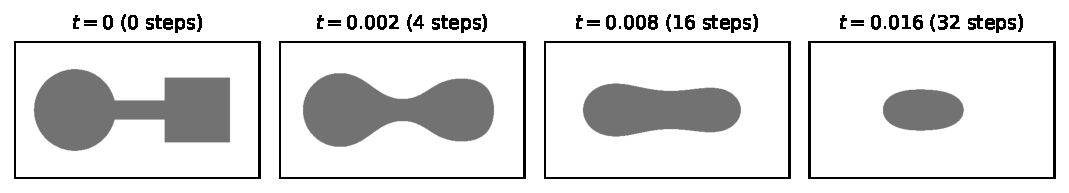
\includegraphics[width=\linewidth]{figures/ch01_dumbbell.pdf}
  \caption{MBO on a non-convex set ($512^2$ grid, $\tau = 5\times10^{-4}$).
  Sharp features are smoothed first; the set becomes convex and shrinks.}
  \label{fig:ch1-dumbbell}
\end{figure}

% =========================================================================
\section{The time step is a two-sided window}
\label{sec:ch1-window}

The only parameter is $\tau$, and on a discrete grid it is squeezed from both
sides. MBO state both constraints \cite[\S4]{merriman1992diffusion}:
\begin{itemize}[nosep]
  \item \textbf{Not too large.} The analysis above needs the blur radius to be
        small compared with the radius of curvature, $\sqrt\tau \ll \rho$.
        Otherwise the blur ``sees'' far-away parts of the set and the motion is
        no longer local.
  \item \textbf{Not too small.} On a grid of spacing $h$, the boundary must move
        at least one grid cell per step, $\kappa\tau \gtrsim h$. Otherwise the
        thresholded set is identical to the old one and the scheme is stuck
        forever. This is called \emph{pinning} or \emph{freezing}.
\end{itemize}
With $\rho = 1/\kappa$ these combine into
\begin{equation}
  \rho\, h \;\lesssim\; \tau \;\ll\; \rho^2 ,
  \qquad\text{or}\qquad
  \sqrt{\rho/h} \;\lesssim\; \sqrt\tau/h \;\ll\; \rho/h .
  \label{eq:ch1-window}
\end{equation}
The window exists only if $\rho \gg h$: features must be well resolved on the
grid.

Figure~\ref{fig:ch1-disc} shows both failures on the same disc. With
$\tau = 2\times10^{-5}$, the displacement per step is $\kappa\tau = 0.04\,h$; the
set never changes, and $R^2$ stays at $0.0625$ for all 1875 steps. With
$\tau = 10^{-2}$, $\sqrt\tau/R_0 = 0.4$; the disc shrinks too fast
($R^2 = 0.0166$ at $t = 0.02$, against $0.0225$ predicted) and is gone after three
steps. Only the middle value tracks the true flow.

\begin{figure}[H]
  \centering
  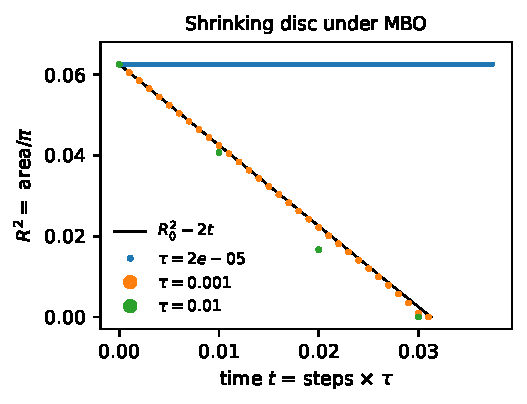
\includegraphics[width=0.55\linewidth]{figures/ch01_shrinking_disc.pdf}
  \caption{A disc of radius $0.25$ under MBO on a $512^2$ grid, against the exact
  law $R^2 = R_0^2 - 2t$. The smallest $\tau$ is pinned (no motion at all), the
  middle one tracks the law, and the largest overshoots.}
  \label{fig:ch1-disc}
\end{figure}

\begin{codebox}
\code{tau\_diagnostics} in \codefile{src/partition/mbo\_auction.py} enforces this
window, with the radius of an equal-area cell
$\Rcell = \sqrt{\text{target area}/\pi}$ standing in for $\rho$ and the mean
edge length $\hmean$ for $h$. The rule is
$\tau = \min\bigl((c\,\hmean)^2,\ (\rho_{\text{cap}}\Rcell)^2\bigr)$, and the
reported lower edge \code{c\_lo\_hmean} $= \sqrt{\Rcell/\hmean}$ is the left
inequality of \eqref{eq:ch1-window} written for $c = \sqrt\tau/\hmean$. Our
diffusion is not a Gaussian (\S\ref{sec:ch1-code}) and moves a boundary by
$\tau\kappa/2$ rather than $\tau\kappa$, so the constants shift by a factor of
order one (\codefile{docs/math/10-mbo-auction-dynamics/} \S5.5; the window
itself is its \S8). The measured window on our meshes is in
\codefile{docs/experiments/08-mbo-auction-dynamics/}.
Why pinning is unavoidable on a discrete domain is van~Gennip et
al.~\cite{vangennip2014mean}, Chapter~5.
\end{codebox}

% =========================================================================
\section{Many phases: the argmax step}
\label{sec:ch1-multiphase}

For a partition into $N$ sets $\Omega_1, \dots, \Omega_N$, MBO 1994
\cite{merriman1994motion} blur every indicator and give each point to the
winner:
\begin{equation}
  u_k = G_\tau * \chi_{\Omega_k}, \qquad
  \omega^{\text{new}}(x) = \argmax_k\, u_k(x) .
  \label{eq:ch1-argmax}
\end{equation}
Because $\sum_k \chi_{\Omega_k} = 1$ and the blur is linear,
$\sum_k u_k = 1$ at every point. With $N = 2$, $u_1 > u_2$ is the same as
$u_1 > \tfrac12$, so \eqref{eq:ch1-argmax} reduces to two-phase MBO. Away from
junctions each interface moves by curvature as before. Where three cells meet,
the scheme produces the junction configuration of the equal-tension network
with no special treatment; equal tensions balance at $120^\circ$.

\paragraph{Experiment E (grid): sixteen cells on a flat torus, no constraint.}
Start from a Voronoi partition of the periodic unit square into 16 cells and run
\eqref{eq:ch1-argmax} with $\tau = 10^{-3}$ on a $256^2$ grid
(Figure~\ref{fig:ch1-multiphase}). Small cells, and cells with few
neighbours, shrink and vanish: 16 cells at step 0, 12 at step 10, 8 at step
100, and a single cell by step 400. \emph{This is correct behaviour.} On a torus,
the partition with the least total boundary is the trivial one, a single cell
with no boundary at all, and unconstrained MBO is heading there. To get $N$ cells of
equal area we must \emph{forbid} cells from shrinking. That constraint is what
Ruuth--Wetton \cite{ruuth2003volume} add for one set and Jacobs--Merkurjev--Esedo\u{g}lu
\cite{jacobs2018auction} add for $N$, and it is the subject of Chapter~3.

\begin{figure}[H]
  \centering
  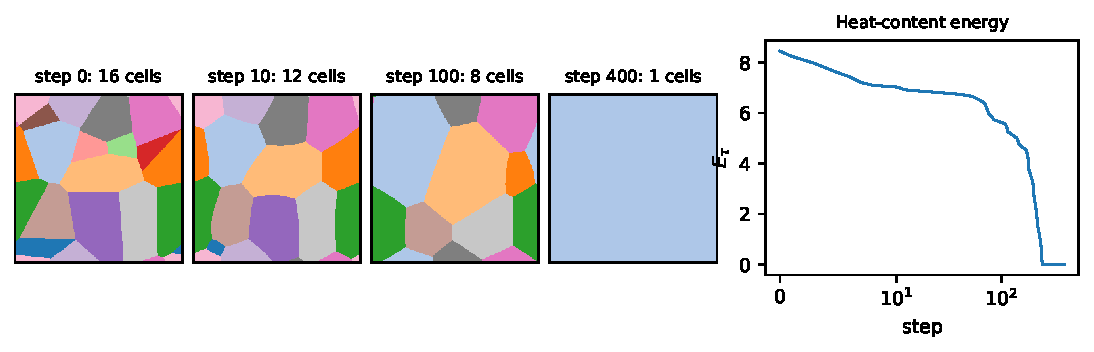
\includegraphics[width=\linewidth]{figures/ch01_multiphase.pdf}
  \caption{Unconstrained multiphase MBO on the flat torus ($256^2$ grid, 16
  Voronoi cells, $\tau = 10^{-3}$). Cells vanish one by one (coarsening). Right:
  the heat-content energy of \S\ref{sec:ch1-energy}, which never increases.}
  \label{fig:ch1-multiphase}
\end{figure}

% =========================================================================
\section{The energy behind the scheme: heat content}
\label{sec:ch1-energy}

So far MBO is an algorithm that happens to approximate a flow. Esedo\u{g}lu and
Otto \cite{esedoglu2015threshold} showed it is something stronger: each step
\emph{minimises} something. This is the view that makes the area constraint easy
to add.

\paragraph{Two phases.}
Heat the set $\Sigma$ to temperature 1, keep the outside at 0, and let heat flow
for time $\tau$. The heat that has left $\Sigma$ is
\begin{equation}
  \Etau(\Sigma) = \frac{1}{\sqrt\tau} \int_\Sigma \bigl(1 - G_\tau * \chi_\Sigma\bigr)\, dA
               = \frac{1}{\sqrt\tau} \int_{\Sigma} G_\tau * \chi_{\Sigma^c}\, dA .
  \label{eq:ch1-heat-content-2}
\end{equation}
Heat leaks out only near the boundary, within a distance of about $\sqrt\tau$, so
this quantity measures boundary length. Make it quantitative on a straight
interface: in the direction normal to the interface, a particle that starts at
depth $s$ inside has crossed it after time $\tau$ if its 1-D displacement $X$
(variance $2\tau$) exceeds $s$. Integrating over the starting depth,
\[
  \text{heat lost per unit length}
  = \int_0^\infty \Pr[X > s]\, ds = \mathbb E[X^+]
  = \frac{\sqrt{2\tau}}{\sqrt{2\pi}} = \sqrt{\frac{\tau}{\pi}} ,
\]
using $\mathbb E[X^+] = \sigma/\sqrt{2\pi}$ for a centred normal with standard
deviation $\sigma$. Dividing by $\sqrt\tau$ gives
\begin{equation}
  \Etau(\Sigma) \;\longrightarrow\; \frac{1}{\sqrt\pi}\, \operatorname{Per}(\Sigma)
  \qquad (\tau \to 0).
  \label{eq:ch1-limit}
\end{equation}
The $1/\sqrt\tau$ in front of \eqref{eq:ch1-heat-content-2} exists to make this
limit finite.

\paragraph{Experiment D (gridless).}
For a disc of radius $0.2$ the limit is $2\pi R/\sqrt\pi = 0.70898$. The exact heat
content divided by that limit is $0.957$, $0.990$, $0.9975$, $0.99937$ and
$0.99984$ at $\sqrt\tau/R = 0.4$, $0.2$, $0.1$, $0.05$ and $0.025$, converging
to~1.

\paragraph{Many phases.}
The natural generalisation adds up the heat each cell loses:
\begin{equation}
  \Etau(\omega) = \frac{1}{\sqrt\tau} \sum_{k=1}^N \int \chi_{\Omega_k}
      \bigl(1 - G_\tau * \chi_{\Omega_k}\bigr)\, dA
  \;\longrightarrow\; \frac{1}{\sqrt\pi}\sum_{k=1}^N \operatorname{Per}(\Omega_k).
  \label{eq:ch1-heat-content-N}
\end{equation}
Every interface between two cells is counted twice, once from each side. This is
the same convention as our project's perimeter $\sum_k \operatorname{Per}(\text{cell}_k)$
(see the standing rule in \codefile{CLAUDE.md}). For $N = 2$ it is twice the
two-phase energy \eqref{eq:ch1-heat-content-2}.

\paragraph{``$\Gamma$-convergence'' in plain words.}
The limit \eqref{eq:ch1-limit} holds for each fixed smooth set. What
optimisation needs is stronger: that \emph{minimisers} of $\Etau$ approach
minimisers of perimeter. $\Gamma$-convergence is the notion of convergence
built to guarantee this. Informally it asks for two things. (i) No cheating from
below: any sequence of sets approaching a shape costs, in the limit, at least
that shape's perimeter. (ii) Every shape's perimeter is achieved: some sequence
approaching the shape has exactly that limiting cost. Esedo\u{g}lu and Otto prove
this for the heat content \cite[App.~A]{esedoglu2015threshold}, and
Esedo\u{g}lu--Jacobs \cite{esedoglu2017kernels} extend it to other kernels. You
can treat the theorem as the licence to say that $\Etau$ is a perimeter.

\begin{physics}
This is the same story as Allen--Cahn / Ginzburg--Landau. The phase-field energy
$\int \varepsilon|\nabla u|^2 + \varepsilon^{-1}W(u)$, with a double-well potential
$W$, $\Gamma$-converges to (surface tension)$\times$(interface length) as the
interface width $\varepsilon \to 0$ (Modica--Mortola \cite{modica1987gradient}). That is the
relaxation Bogosel--Oudet use, and so it is what our PGD Phase~1 minimises. The
heat content is a \emph{nonlocal} cousin, with interface width $\sqrt\tau$ in
place of $\varepsilon$. Both methods minimise a surrogate for perimeter. The
difference is the variable: PGD optimises a fuzzy density and must read a
partition off at the end, while MBO only ever holds a partition.
\end{physics}

% =========================================================================
\section{Each MBO step is a descent step}
\label{sec:ch1-descent}

This section is the bridge to auction dynamics, so it is worth understanding
fully. It needs only two inequalities.

\paragraph{Relax.}
Let the cells be ``soft'': $u = (u_1, \dots, u_N)$ with $u_k(x) \ge 0$ and
$\sum_k u_k(x) = 1$ at each point (a probability vector per point). Write the
energy for such $u$. Since $\sum_k \int u_k = |\Omega|$ (the total area),
\begin{equation}
  \Etau(u) = \frac{1}{\sqrt\tau}\Bigl[\,|\Omega| - \sum_k \int u_k\, (G_\tau * u_k)\,dA\Bigr].
  \label{eq:ch1-relaxed}
\end{equation}
For hard indicators this is exactly \eqref{eq:ch1-heat-content-N}.

\paragraph{It is concave.}
By Parseval, $\int f\,(G_\tau * f) = (2\pi)^{-d}\int \widehat{G_\tau}(\xi)\,
|\hat f(\xi)|^2\, d\xi \ge 0$, because $\widehat{G_\tau} = e^{-\tau|\xi|^2} > 0$.
So each term $\int u_k\, G_\tau * u_k$ is a positive quadratic form in $u_k$, a
bowl. Since it enters with a minus sign, $\Etau$ is an upside-down bowl:
\emph{concave}. This is property~4 of \S\ref{sec:ch1-heat} at work.

\paragraph{Linearise.}
At the current partition $u$, the tangent-plane approximation of $\Etau$ is
\[
  L_u(u') = \Etau(u) + \bigl\langle \nabla \Etau(u),\, u' - u \bigr\rangle,
  \qquad \nabla_{u_k} \Etau(u) = -\frac{2}{\sqrt\tau}\, G_\tau * u_k ,
\]
using the symmetry of $G_\tau$ (property~3). Apart from constants, minimising
$L_u$ means maximising $\sum_k \int u'_k\, (G_\tau * u_k)$ over probability
vectors $u'$. This decouples point by point. At each $x$, put all the weight
on the largest $(G_\tau * u_k)(x)$. \textbf{That is exactly the argmax step}
\eqref{eq:ch1-argmax}. So an MBO step is ``minimise the tangent plane of the
energy''.

\paragraph{Descend.}
For a concave function, the tangent plane lies \emph{above} the graph
everywhere. So, with $u'$ the MBO update,
\begin{equation}
  \Etau(u') \;\le\; L_u(u') \;\le\; L_u(u) \;=\; \Etau(u).
  \label{eq:ch1-descent}
\end{equation}
The first inequality is concavity. The second holds because $u'$ minimises $L_u$
and $u$ is one of the candidates. Hence \textbf{the energy never increases},
for any $\tau$, with no step-size control. This is Esedo\u{g}lu--Otto's Lemma~5.2
in our notation \cite{esedoglu2015threshold}. On the grid of Experiment~E the
FFT blur also has a positive multiplier, so the argument applies verbatim. The
measured energy falls from $8.46$ to $0$, and no step increases it
(Figure~\ref{fig:ch1-multiphase}, right).

\begin{keyidea}[title={Key idea: why this is the door to auction dynamics}]
The second inequality in \eqref{eq:ch1-descent} used only that the current
partition $u$ is \emph{one of the allowed candidates}. So add any constraint the
current partition already satisfies, such as ``every cell has area $A$'', and
minimise $L_u$ over the constrained candidates. The energy still cannot
increase, provided the constrained problem is solved \emph{exactly}. The price
is that the problem no longer decouples point by point: the cells compete for a
fixed budget of area. Chapter~3 shows that it becomes a classical
\emph{assignment problem}. Its solution is a shifted argmax
$\argmax_k\,[u_k(x) + \psi_k]$, where each $\psi_k$ is a Lagrange multiplier,
a ``price'' for cell $k$.
\end{keyidea}

\begin{physics}
The $\psi_k$ are chemical potentials. Fixing each cell's area is like fixing
each species' particle number. Lagrange multipliers turn the constrained
(canonical) problem into an unconstrained (grand-canonical) one, and the
multiplier is set so that the average particle number comes out right. A cell
that is too small raises its $\psi_k$ and attracts points; a cell that is too
large lowers it.
\end{physics}

% =========================================================================
\section{From the flat torus to our code}
\label{sec:ch1-code}

\begin{center}
\small
\begin{tabular}{@{}p{0.36\linewidth}p{0.58\linewidth}@{}}
\toprule
In this chapter & In \codefile{src/partition/mbo\_auction.py} \\
\midrule
Indicators $\chi_{\Omega_k}$ &
  \code{sparse\_one\_hot(labels, n\_cells)}; the state is a vertex labelling \\
Blur $G_\tau * \chi_k$ (exact heat flow) &
  \code{diffuse\_indicators}: solve $(M + \tau K)\,y_k = M\chi_k$ for each $k$,
  one backward-Euler step of $M\dot y + K y = 0$, with $M$, $K$ the P1 mass and
  stiffness matrices \\
Argmax \eqref{eq:ch1-argmax} &
  \code{balanced\_assign}: the \emph{shifted} argmax $\argmax_k[y_{ik} + \psi_k]$
  with equal-area prices (Chapter~3) \\
Heat content \eqref{eq:ch1-relaxed} &
  \code{lyapunov\_energy}: $(|S| - \sum_k \chi_k^\top \Dlump\, y_k)/\sqrt\tau$, the
  same formula with integrals replaced by lumped-mass sums \\
Descent inequality \eqref{eq:ch1-descent} &
  \code{descent\_slack}: what survives of it when the assignment is solved
  inexactly (\codefile{docs/math/10-mbo-auction-dynamics/} \S7) \\
Time-step window \eqref{eq:ch1-window} &
  \code{tau\_diagnostics} \\
\bottomrule
\end{tabular}
\end{center}

\paragraph{Why our blur is not a Gaussian, and why that is fine.}
On a triangulated surface there is no FFT. The code takes one implicit-Euler
step of the heat equation, $(I - \tau\Delta)^{-1}$ in continuum notation, rather
than the exact flow $e^{\tau\Delta}$. In Fourier language the multiplier is
$1/(1 + \tau|\xi|^2)$ instead of $e^{-\tau|\xi|^2}$. The two agree for long
wavelengths, and both are \emph{positive}, so the concavity argument of
\S\ref{sec:ch1-descent} survives. There is also a neat identity,
\[
  \frac{1}{1 + \tau|\xi|^2} = \int_0^\infty e^{-s}\, e^{-s\tau|\xi|^2}\, ds ,
\]
which says that one implicit step is an \emph{average of exact heat flows} over
random times $s\tau$ with $s$ exponentially distributed. Averaging
\eqref{eq:ch1-displacement} and \eqref{eq:ch1-limit} over those times is how
\codefile{docs/math/10-mbo-auction-dynamics/} \S5.2--5.5 obtains our kernel's constants
(per-step displacement $\tau\kappa/2$, interface constant $\tfrac12$ in place of
$1/\sqrt\pi$). This is also why Esedo\u{g}lu--Jacobs \cite{esedoglu2017kernels}, on kernels
other than the Gaussian, matters to us (Chapter~4).

% =========================================================================
\section{Exercises}
\label{sec:ch1-exercises}

Short, and meant to be done with pencil or with the script.
\begin{enumerate}
  \item From $dR/dt = -1/R$, derive \eqref{eq:ch1-disc}. A square of side $a$ under
        curvature flow: when does it vanish? (Hint: use $dA/dt = -2\pi$, not the
        shape.)
  \item Show $\mathbb E[X^+] = \sigma/\sqrt{2\pi}$ for $X \sim N(0, \sigma^2)$, and
        recover the constant $1/\sqrt\pi$ in \eqref{eq:ch1-limit}.
  \item In one dimension a ``set'' is an interval of length $\ell$. Show that
        two-phase MBO with $\sqrt\tau \ll \ell$ moves its endpoints by an amount
        that is exponentially small in $\ell^2/\tau$. (There is no curvature in
        1-D; only the far endpoint is felt.) What happens when $\ell \lesssim \sqrt\tau$?
  \item Threshold at $0.4$ instead of $\tfrac12$. How does a flat interface move
        now, and how far per step? You have just added a pressure term.
        Ruuth--Wetton \cite{ruuth2003volume} choose the threshold \emph{at every
        step} so that the area is preserved. That is the one-cell version of the
        prices $\psi_k$.
  \item Check that for $N = 2$, \eqref{eq:ch1-heat-content-N} equals twice
        \eqref{eq:ch1-heat-content-2}.
  \item With the script, lower $\tau$ in experiment~B step by step and locate the
        pinning threshold on the $512^2$ grid. Compare it with $\kappa\tau \approx h$.
\end{enumerate}

% =========================================================================
\section{Summary}

\begin{itemize}[nosep]
  \item Curvature flow is the steepest descent of boundary length
        \eqref{eq:ch1-dLdt}.
  \item MBO computes it by \emph{blur, then threshold at $\tfrac12$}. Each step moves
        the boundary by $\kappa\tau$ \eqref{eq:ch1-displacement}, and $\tau$ must sit
        in a two-sided window \eqref{eq:ch1-window}.
  \item With $N$ cells the threshold becomes an argmax \eqref{eq:ch1-argmax}.
        Left alone, cells vanish, because fewer cells means less boundary.
  \item MBO minimises the tangent plane of a concave heat-content energy
        that converges to the total perimeter, so it never increases that energy
        \eqref{eq:ch1-descent}. The argument tolerates any constraint the current
        partition already satisfies, which is how the equal-area constraint enters
        in Chapter~3.
\end{itemize}


\bibliographystyle{plain}
\bibliography{../math/shared/references,study}

\end{document}
